\documentclass{beamer}
\usetheme{Darmstadt}
\usecolortheme{wolverine}
\usepackage{tikz, graphicx}

\title{Using Twitter to Predict Cryptocurrency}
\author[Claudeon]{Claudeon Reinard Susanto \\ \texttt{claudeon.susanto@u.nus.edu}}
\date[11 Nov '22]{Friday, 11 November 2022}
\begin{document}
\begin{frame}[plain]
    \maketitle
\end{frame}

\begin{frame}[plain]
	\frametitle{Outline}
	\tableofcontents[hideothersubsections]
\end{frame}

\section{Problem}
\begin{frame}
	\frametitle{Outline}
	\tableofcontents[hideothersubsections]
\end{frame}

\subsection{Introduction to cryptocurrency}
\begin{frame}
	\frametitle{Cryptocurrency is a form of digital currency that is secured using cryptography}
	\begin{columns}[t]
		\begin{column}{0.3\textwidth}
			content...
		\end{column}
	\begin{column}{0.05\textwidth}
		+
	\end{column}
	\begin{column}{0.3\textwidth}
		content...
	\end{column}
\begin{column}{0.05\textwidth}
	$\rightarrow$
\end{column}
\begin{column}{0.3\textwidth}
	content...
\end{column}
	\end{columns}
\end{frame}
\begin{frame}
	\frametitle{Cryptocurrency is faster and more secure than digital cash}
\end{frame}
\begin{frame}
	\frametitle{Cryptocurrencies are slowly replacing digital currency}
\end{frame}
\begin{frame}[plain]
	\centering \Large{Hopefully I have convinced you to start investing in crypto...}
\end{frame}
\subsection{Cryptocurrency's volatility}
\begin{frame}
	\frametitle{Cryptocurrency prices are highly volatile}
\end{frame}
\begin{frame}
	\frametitle{Volatile prices make it very difficult for potential \textbf{buyers} and sellers to make decisions}
\end{frame}
\begin{frame}
	\frametitle{Volatile prices make it very difficult for potential buyers and \textbf{sellers} to make decisions}
\end{frame}
\subsection{Limitations of past studies}
\begin{frame}
	\frametitle{Previous methods to predict cryptocurrency prices are ineffective, slow, and }
	\begin{columns}[t]
		\begin{column}<1->{0.333\textwidth}
			\begin{figure}[H]
				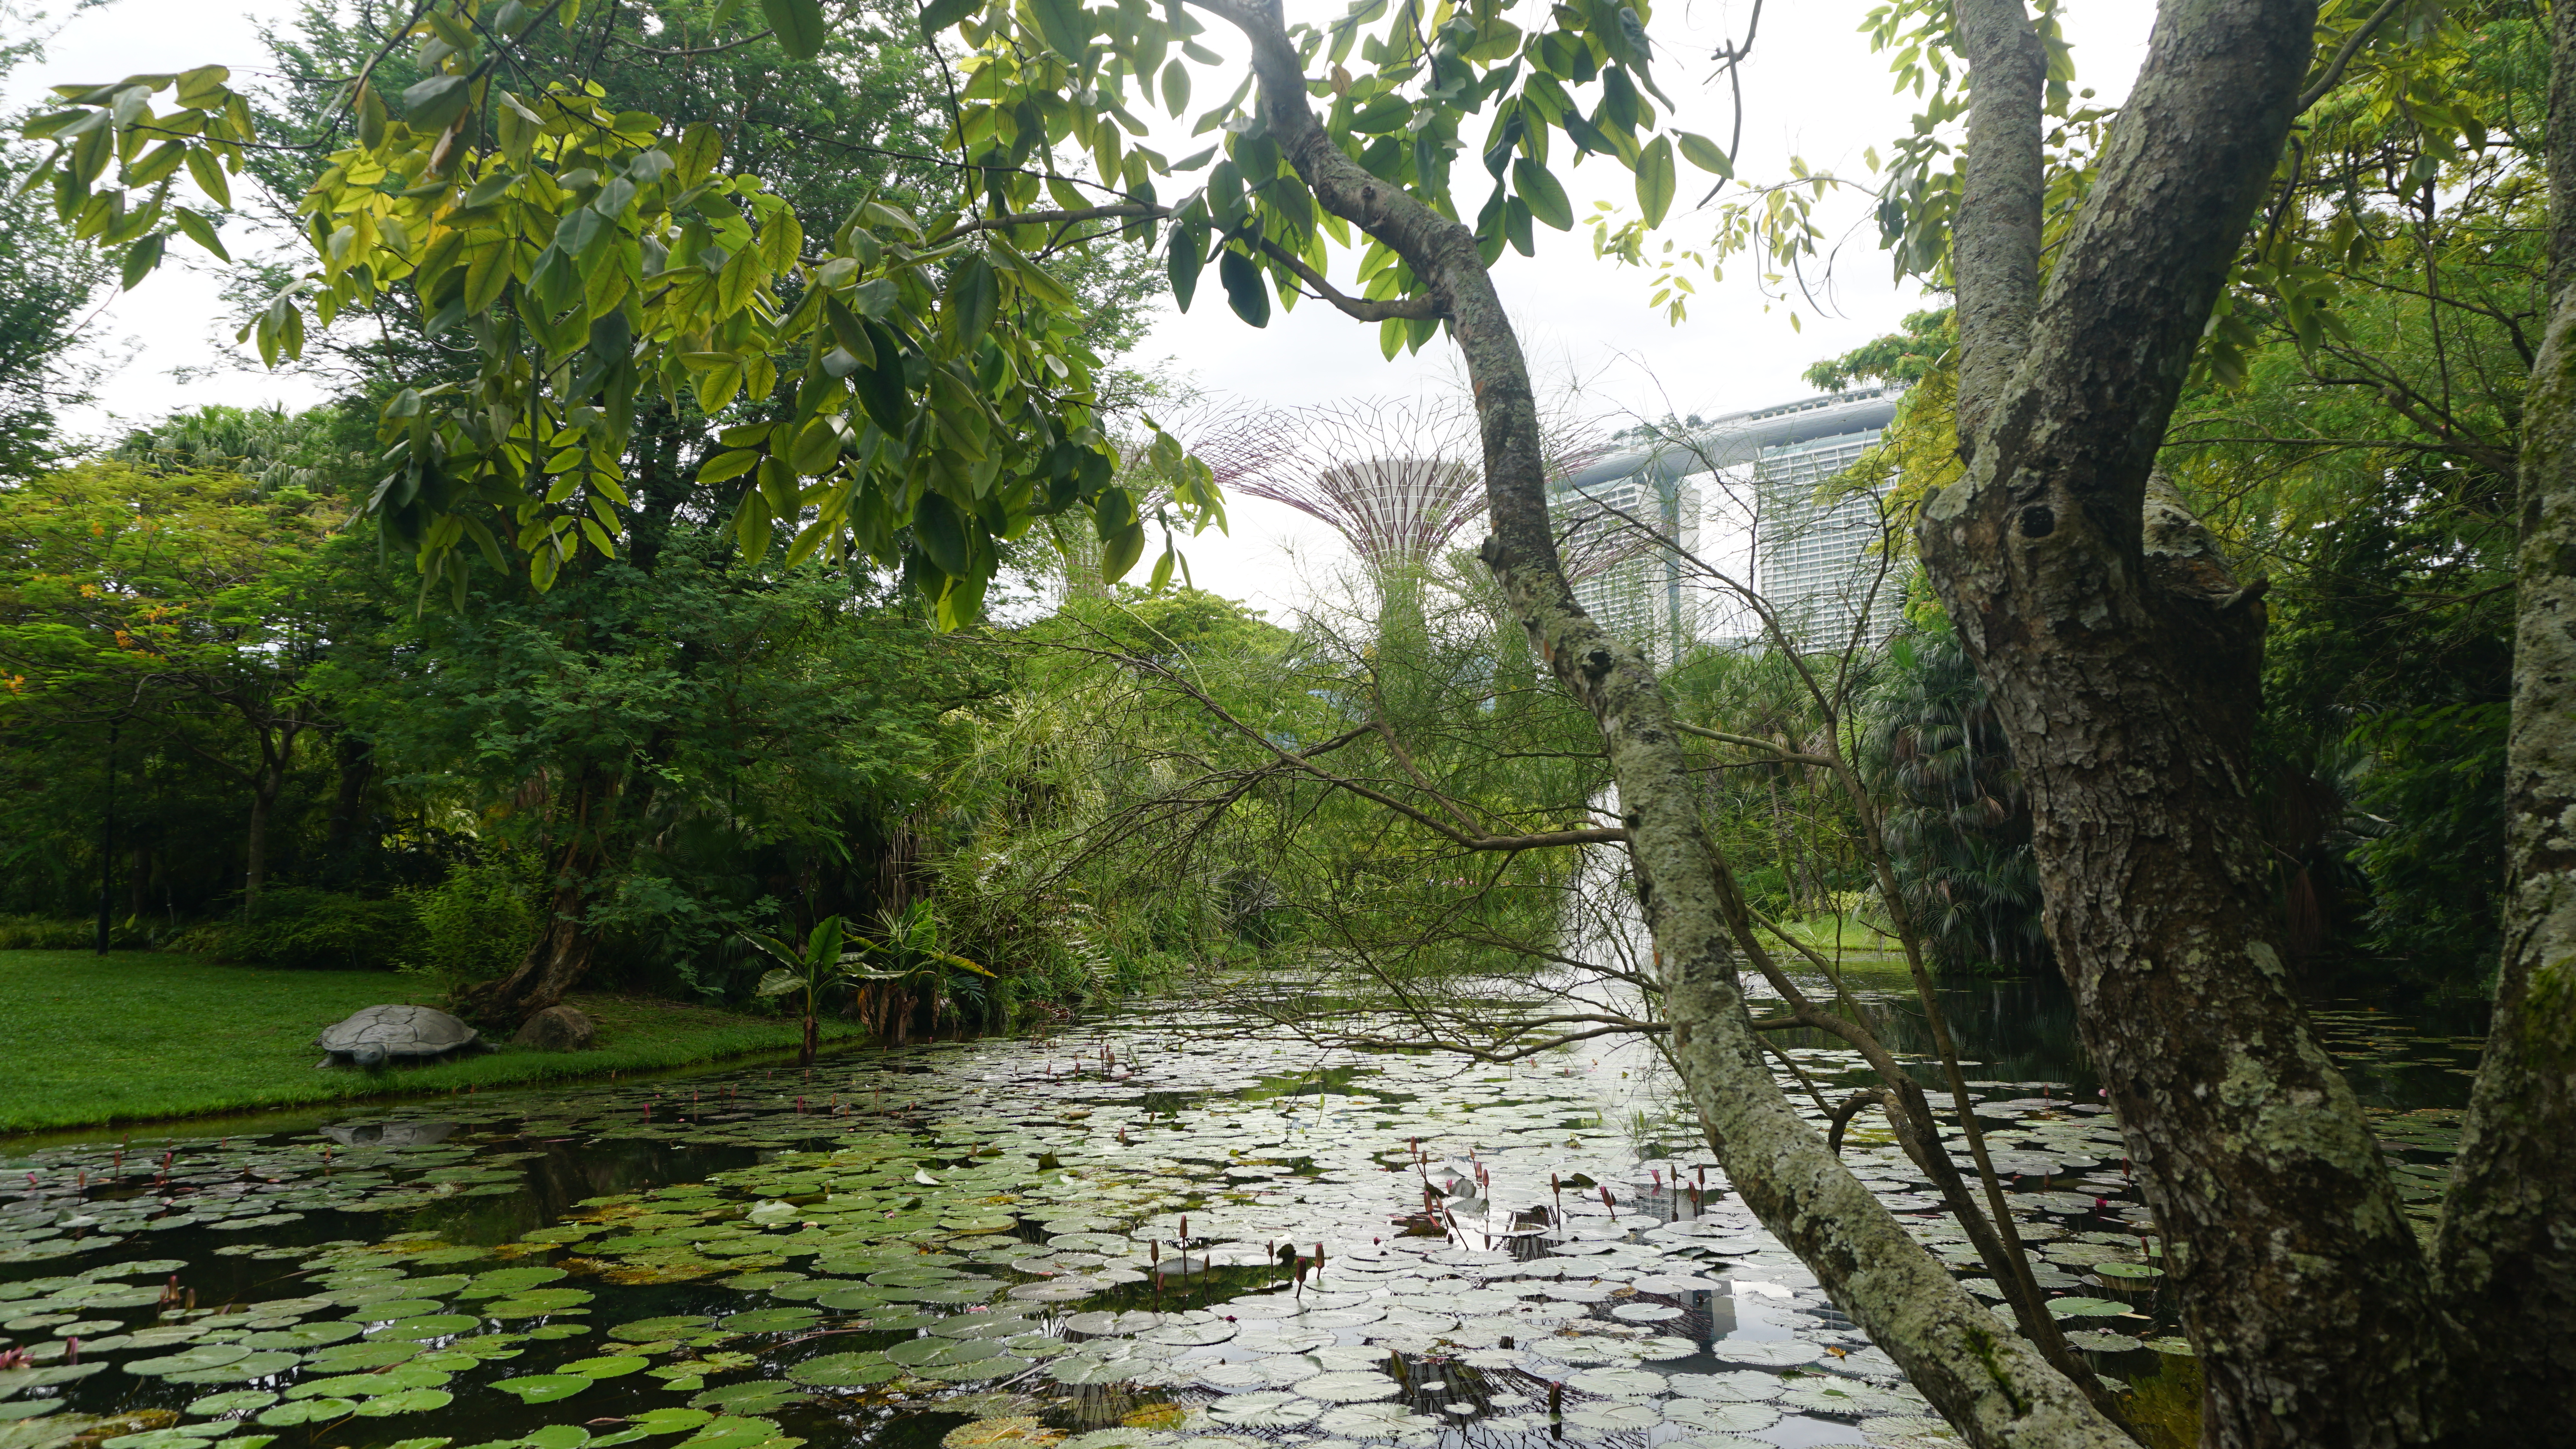
\includegraphics[width=\columnwidth]{images/DSC02384.JPG}
			\end{figure}
		    \centering ineffective
		\end{column}
		\begin{column}<2->{0.333\textwidth}
			\begin{figure}[H]
				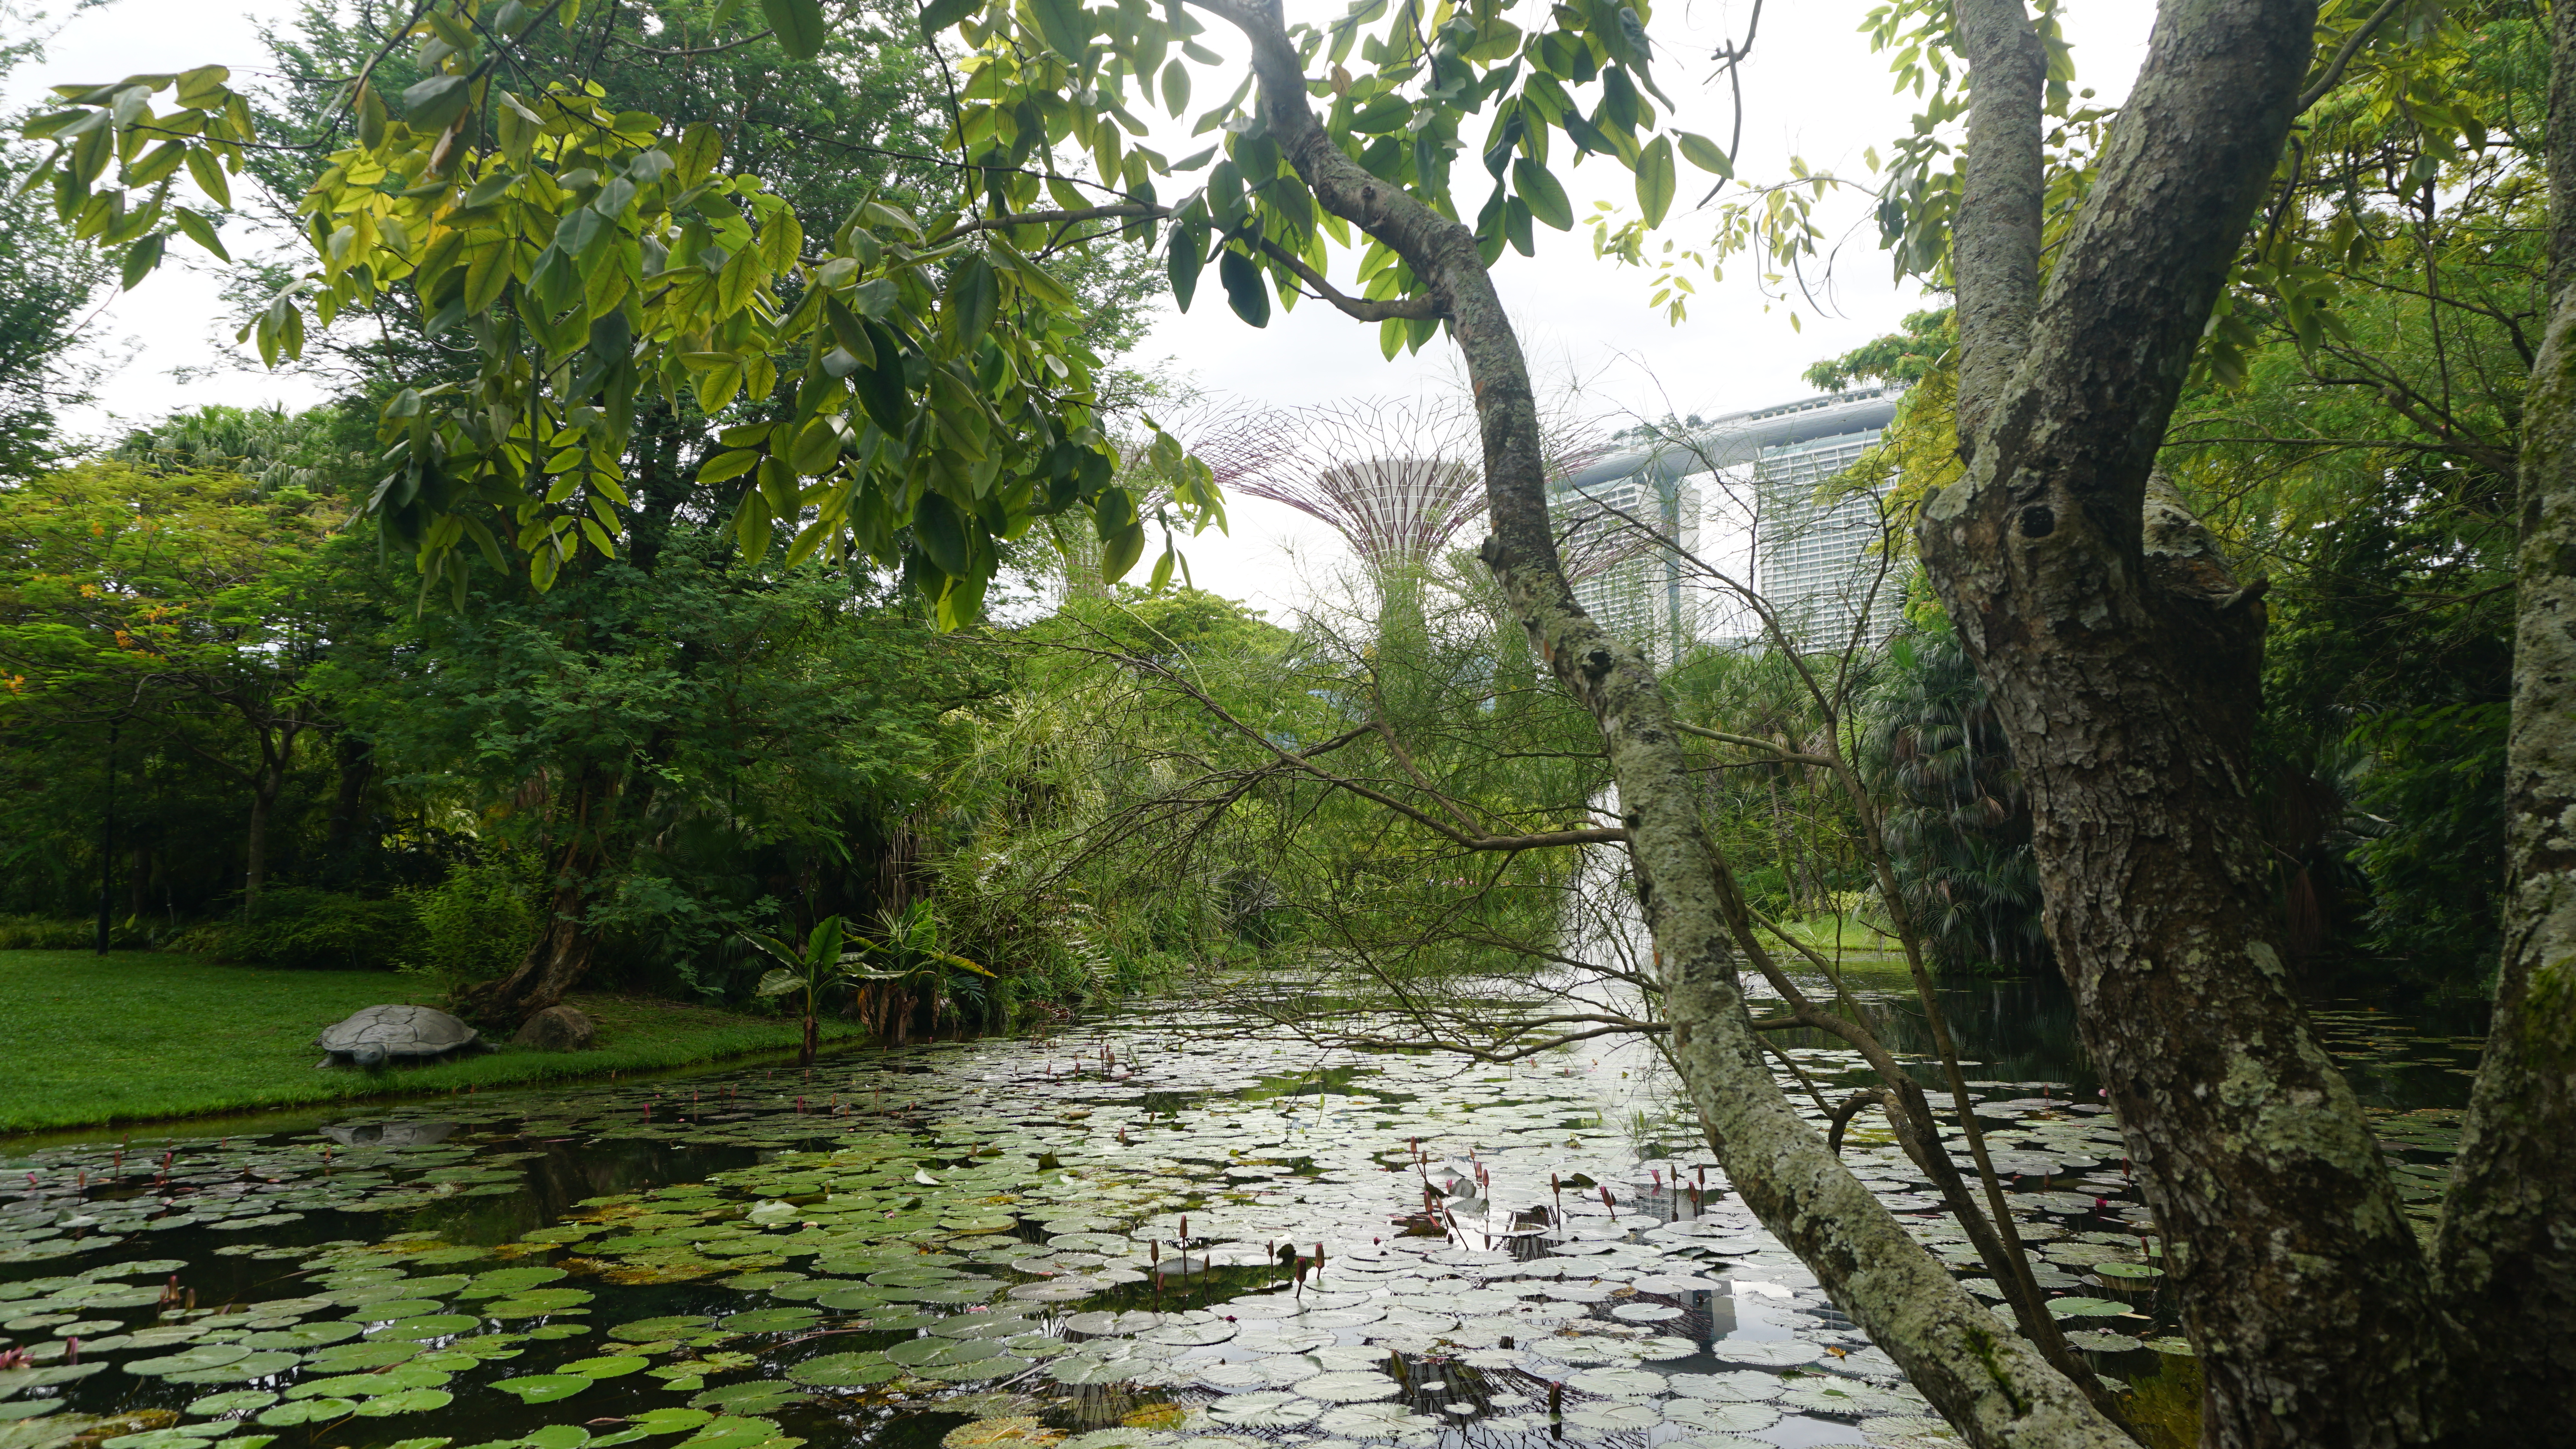
\includegraphics[width=\columnwidth]{images/DSC02384.JPG}
			\end{figure}
		\end{column}
		\begin{column}<3->{0.333\textwidth}
			\begin{figure}[H]
				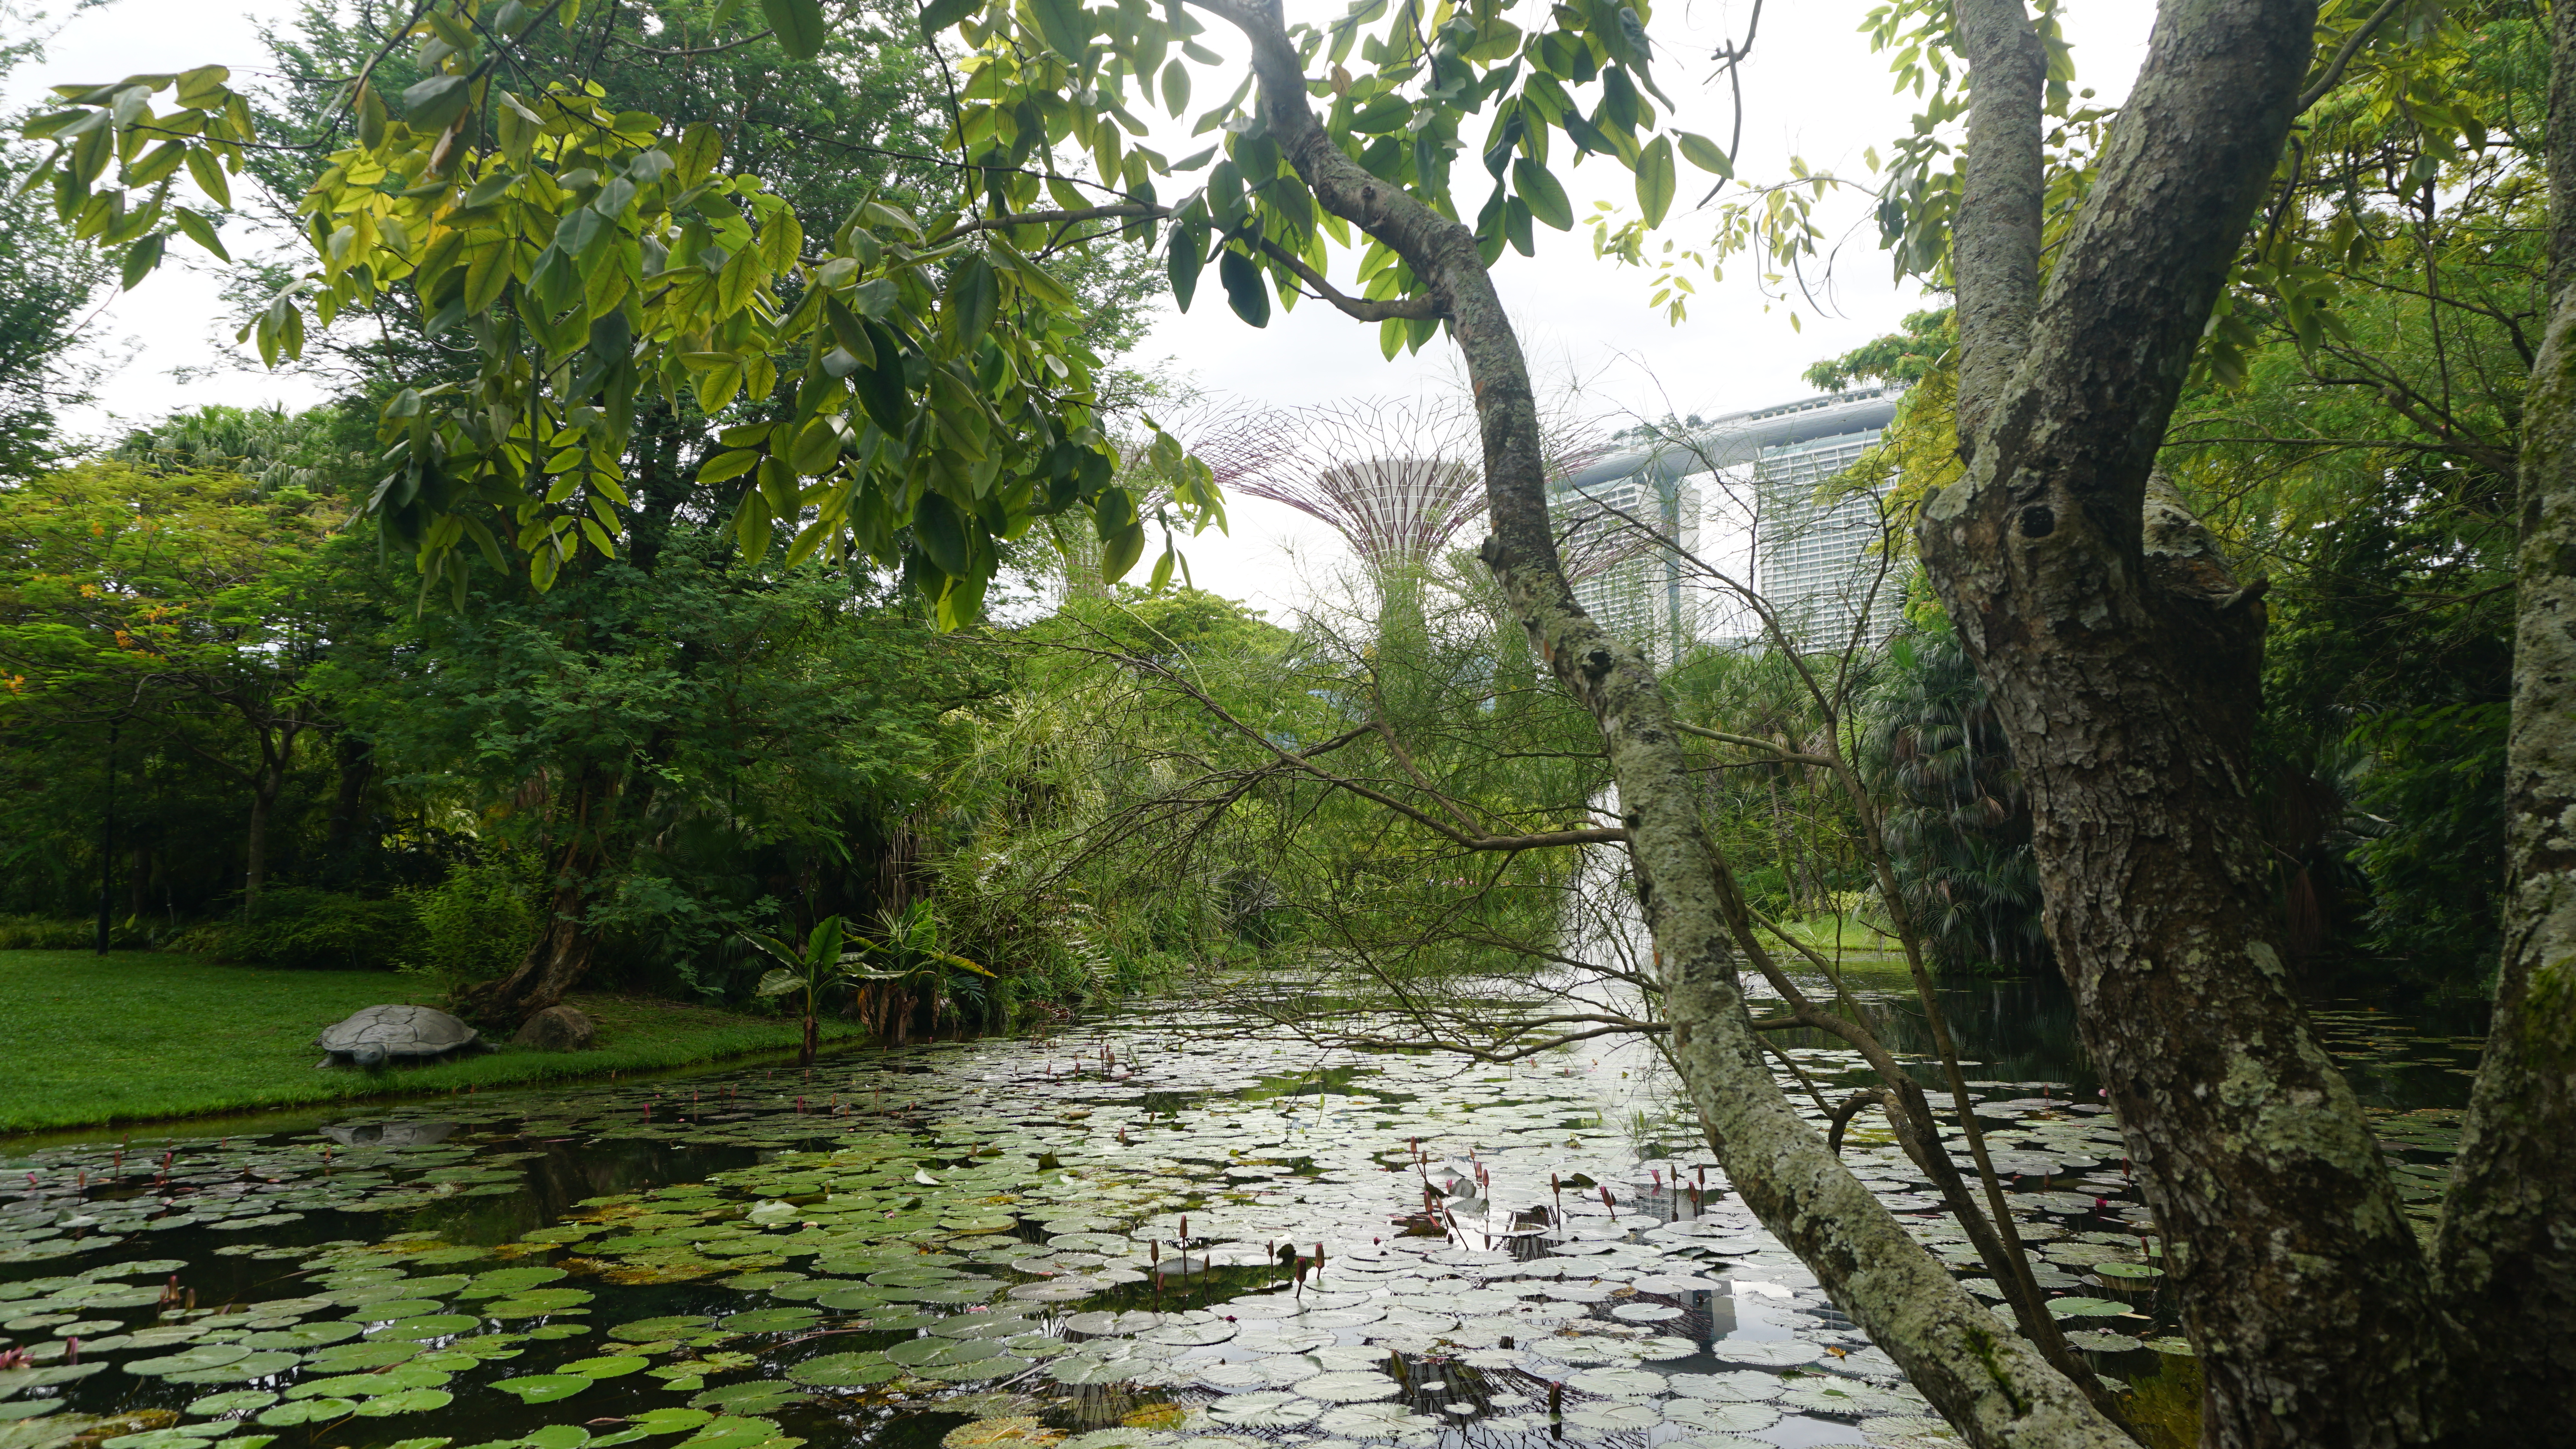
\includegraphics[width=\columnwidth]{images/DSC02384.JPG}
			\end{figure}
		\end{column}
	\end{columns}
\end{frame}
\section{Solution}
\begin{frame}
	\frametitle{Outline}
	\tableofcontents[hideothersubsections]
\end{frame}
\subsection{Twitter data and cryptocurrency}
\begin{frame}
	\frametitle{Twitter data can be easily obtained and provide real-time updates of current market conditions}
\end{frame}
\begin{frame}
	\frametitle{YAY}
\end{frame}
\subsection{Methodology}
\subsection{Results}

\section{Discussion}
\subsection{Limitations}
\begin{frame}
	\frametitle{Outline}
	\tableofcontents[hideothersubsections]
\end{frame}
\begin{frame}
	\frametitle{Confirmed the claim that this}
\end{frame}
\begin{frame}
	\frametitle{Data collected over a short 2-months period; might be inaccurate}
\end{frame}
\subsection{Applications}
\subsection{Future Research}
\begin{frame}[plain]
	\frametitle{Bibliography}
	\begin{thebibliography}{Dijkstra, 1982}
		\bibitem[Salomaa, 1973]{Salomaa1973}
		A.~Salomaa.
		\newblock {\em Formal Languages}.
		\newblock Academic Press, 1973.
		\bibitem[Dijkstra, 1982]{Dijkstra1982}
		E.~Dijkstra.
		\newblock Smoothsort, an alternative for sorting in situ.
		\newblock {\em Science of Computer Programming}, 1(3):223--233, 1982.
	\end{thebibliography}
\end{frame}

\end{document}
